%===================================== CHAP 3 =================================

\chapter{Project Management}
This chapter includes a description of the methodology and how this was completed throughout the project. Furthermore, it includes the team organization and the risk analysis.

\section{Methodology}
\label{methodology}
During the development of the product the group decided to utilize Scrum and the agile methodology. This was a natural choice of methodology as the customer required the process to be iterative, based on the group's previous experiences and the research completed. 

The process methodology was adjusted to suit the project in the best possible manner, as well as to suit the group's needs. The group completed daily meetings, sprint reviews and sprint retrospectives to achieve the best possible outcome of the project. To maintain consistent communication with the customer, scheduled meetings were weekly held having the opportunity for more if needed. 

During the development process, the group also utilized some principles from Extreme Programming, specifically the practice of pair programming. A decision based upon the groups desire to maximize the learning opportunities from each other, resulting in the best possible outcome. As the productivity was increased by efficiently sharing knowledge and discussing problems, the quality of the code was subsequently improved.  

\subsection{Development}
Throughout the development the group utilized the practice of issue tracking on GitHub, and structured the tasks based on milestones. To ensure that the group followed the principles of Scrum, the milestones were used as a base for sprint planning. To easily track the issues during the development the group used Waffle.io as a Scrum board. This provided the group a visualization of the process in real time, with issues in 'product backlog', 'sprint backlog' and 'in process' including who was working on which, using assignees. 

\subsection{Report}
Waffle.io was also used during the process of writing the report. Primarily to ensure that every member participated in writing and proof-reading parts of the report.

\section{Team Organization}
\label{projectOrganisation}
The group decided to divide the project into reasonable areas of development, and delegated the main responsibility to two or more of the group members, where one had the main responsibility. This would ensure that all parts of the project were kept in mind during the development, as well as more than one person knew what was going on in one specific area.

\subsubsection{Scrum Master}
\textit{Responsible: Ingrid Skar} \\
Skar was given the role as Scrum Master due to previous experience with leading a team and the coordination of Scrum related tasks. This included coordinating work packages, sprints and milestones.

\subsubsection{Group Leader}
\textit{Responsible: Christina Hellenes Andresen} \\
Andresen became group leader through a vote within the group. The role as group leader included having an overview of the project status, attending group leader meetings, create meeting agendas and lead the daily meetings.  

\subsubsection{Contact Responsible}
\textit{Responsible: Sigve André Evensen Skaugvoll} \\
Skaugvoll was selected as the responsible person for keeping contact with both customer and supervisor. The contact responsible acted as a link between the group, the customer and the supervisor, arranging meetings and making sure both parts got the meeting agenda before the meetings.

\subsubsection{Architect}
\textit{Responsible: Martin Stigen} \\
The role of architect was given to Stigen, due to interests and experience. The architect was responsible for providing an initial draft of the architecture and for integrating the backend together with the frontend. Skaugvoll was also a part of the architect team.

\subsubsection{Database}
\textit{Responsible: Andreas Norstein}\\
Norstein was assigned the main responsibility for the database given his previous experiences from courses at QUT. The responsibility included investigating the different options, requirements for the database and create entity relation diagram. Norstein had this responsibility together with Skaugvoll.

\subsubsection{Backend}
\textit{Responsible: Sigve André Evensen Skaugvoll}\\
The main responsibility for this role was investigating the backend options and setting up the project server. Skaugvoll worked together with Norstein after the group had decided on using Django as the backend. Skaugvoll and Norstein were elected based on some prior experience through own projects, course at NTNU and interests.

\subsubsection{Frontend}
\textit{Responsible: Thomas Wold}\\
Wold was given the role as frontend responsible, mainly because of experiences with frontend development from courses he had attended at NTNU. This responsibility was shared with Skar and Stigen. Their work included choosing development languages, frameworks and libraries, as well as preparing the development environment.

\subsubsection{Interaction Designer}
\textit{Responsible: Ingrid Skar}\\
The interaction designer was responsible for creating the paper prototype and styling the product. Skar was given the main responsibility for this task, together with Andresen, mainly because of their interest in the field.

\subsubsection{Testing}
\textit{Responsible: Christina Hellenes Andresen}\\
Andresen was given the role as tester, this included setting up a test plan- and strategies. Skaugvoll and Skar were co-responsible for testing. These three also prepared for the workshops and focus groups.

\subsubsection{Report}
\textit{Responsible: Christina Hellenes Andresen}\\
Andresen was given the role of report responsible, due to previous experience. This role included setting up the table of content and keeping the report backlog updated on Waffle.io. Wold was also a part of this team.

\section{Work Breakdown Structure}
The project activities were divided into manageable sections, defined as work packages (see figure \ref{Work_Breakdown_Structure}). By outlining the project and organizing it into smaller sections, the group got a better overview of what was expected to be developed.

\begin{figure}[ht]
\centering
    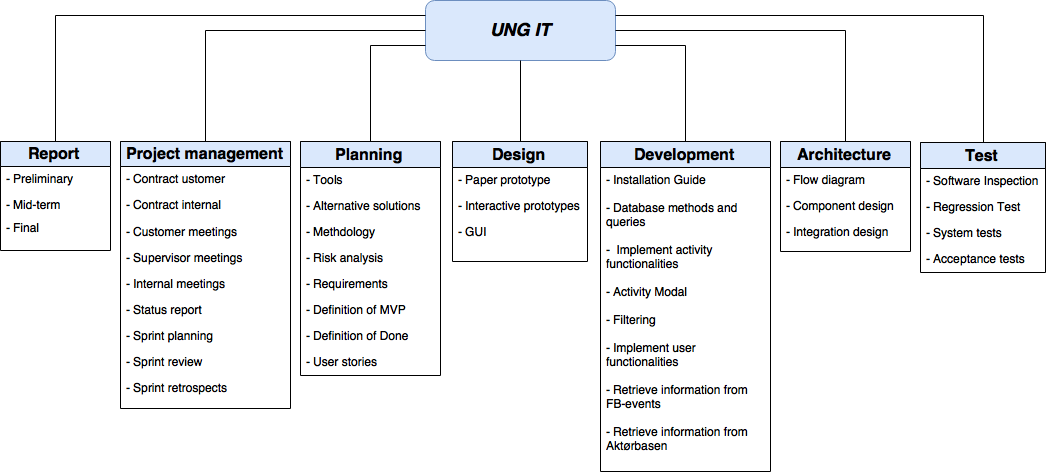
\includegraphics[width=1\textwidth]{fig/work_packages_new}
\caption{Work Breakdown Structure}
\label{Work_Breakdown_Structure}
\end{figure}

\subsection{Gantt Diagram} \label{GanttDiagram}
The project's life cycle was visualized using a Gantt Diagram (see figure \ref{Gantt_Diagram}). This was useful while planning the development process, as the group got a common understanding of what should be done in which phase, and could delegate resources based on this. 

The model reflects how the group worked following the agile methodologies. The development was divided into sprints lasting two weeks. The life cycle of the other work packages depended on the scope; some lasted throughout the entire project, such as the project management, and others occurred in specific phases, such as planning or testing. 


\begin{center}
  \makebox[\textwidth]{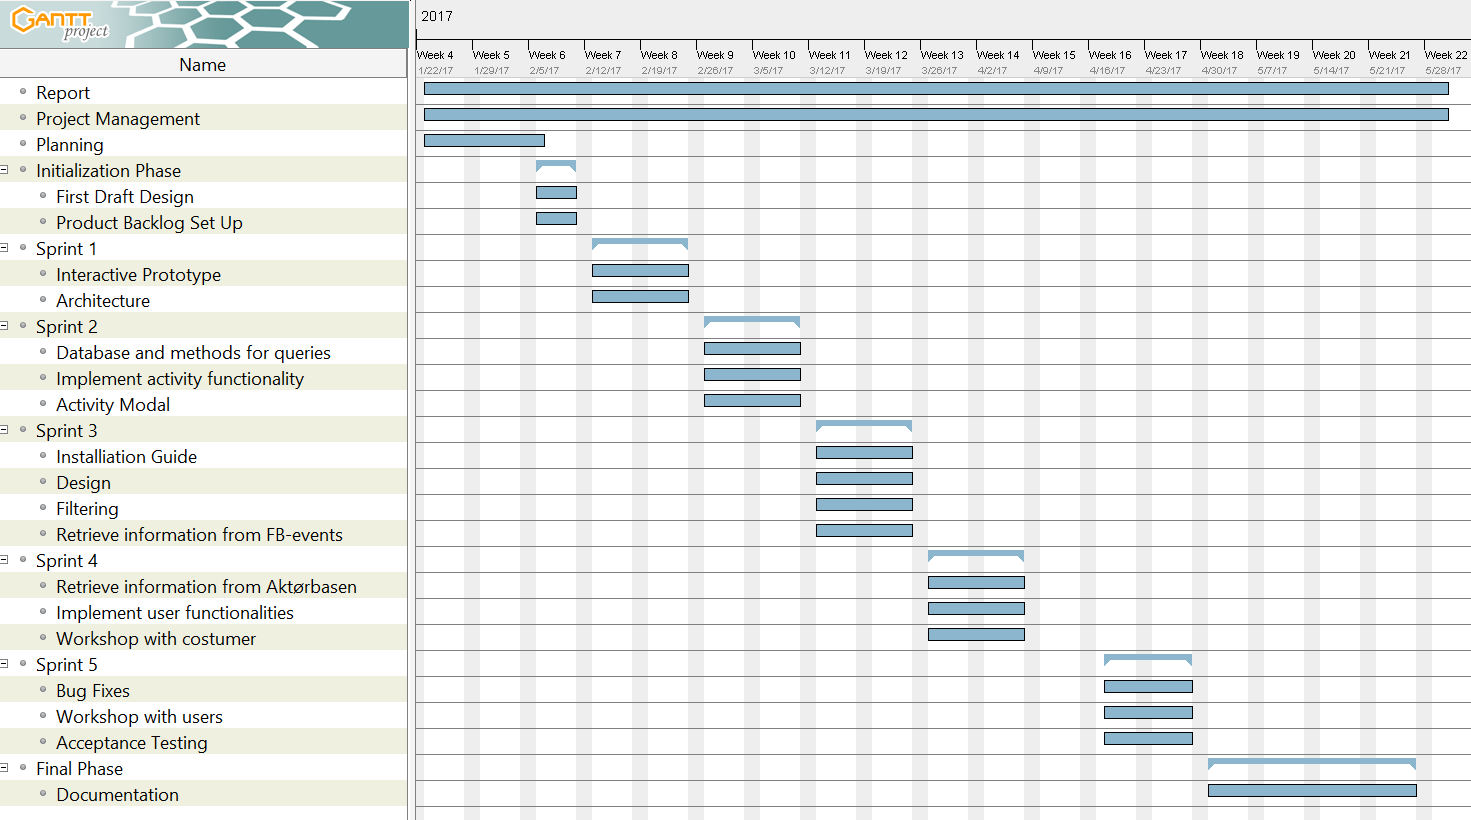
\includegraphics[angle=90,height=150mm,width=\linewidth]{fig/GanttDiagram.PNG}}
  \begin{figure}[!h]
    \caption{Gantt Diagram}
    \label{Gantt_Diagram}  
  \end{figure}
\end{center}


\section{Milestones}
\label{milestones}
The milestones in the project were defined by the main features requested by the customer. These included a group of issues corresponding to the features the milestone disclosed, in accordance to GitHub's guidelines \cite{GitHubGuide}. Furthermore, the milestone did also consist of important events, such as user testing and delivery of project. 
 
\begin{longtable}{@{\extracolsep{\fill}}
                |L{0.10\linewidth}
                |L{0.15\linewidth}
                |L{0.65\linewidth}|@{}}
\hline
\rowcolor{Gray}
\textbf{Date} & \textbf{Milestone} & \textbf{Theme} \\
\hline
\textbf{10.02} & Milestone 0 & Create first draft of design, plan and set up preliminary version of product backlog, and set up development environment \\
\hline
\textbf{15.02} & Report & Preliminary delivery of report \\
\hline
\textbf{24.02} & Milestone 1 & Create skeleton of product, design and overview of activities, define user specifications.  \\
\hline
\textbf{03.03} & Milestone 2 & Database and methods for queries.\\
\hline
\textbf{17.03} & Milestone 3 & User interaction, and create installation guide. \\
\hline
\textbf{19.03} & Report & Mid semester version of report\\
\hline
\textbf{21.03} & Milestone 4 & User testing \\
\hline
\textbf{07.04} & Milestone 5 & Group deadline. No new features should be implemented. \\
\hline
\textbf{11.05} & & Final Presentation \\
\hline
\textbf{30.05} & & Delivery  \\
\hline
\caption{Milestones}
\label{Milestones}
\end{longtable}


\section{Sprints}
\label{s:sprints}
The group divided the development process into sprints (see table \ref{t:sprints}), were each sprint lasted for two weeks, running from Monday to Friday the next week. Each sprint was planned with respect to the given milestones. During a sprint, the group arranged workdays and group meetings, to plan and work on the project. 

In order to follow the chosen methodology the group arranged meetings with the costumer each Wednesday from Sprint one to Sprint five, and completed Sprint Reviews. The meetings were informal and facilitated for close cooperation with the customer.

At the end of each sprint the group completed a Sprint retrospective; were each member reflected over the past sprint, and suggested actions to improve to the upcoming sprint. This allowed each member to individually express how they thought the development was progressing, as well as how to further develop as a group. 

\begin{longtable}{@{\extracolsep{\fill}}
                |L{0.16\linewidth}
                |L{0.18\linewidth}
                |L{0.12\linewidth}
                |L{0.40\linewidth}|@{}}
               
\hline
\rowcolor{Gray}
\textbf{Dates}&\textbf{Planned Work Hours}&\textbf{Sprint}&\textbf{Goal}\\
\hline
06.02 - 10.02&136.5&Sprint 0&Initialization phase. Planning, product backlog set up and first draft design.\\
\hline
13.02 - 24.02&270&Sprint 1& Deliver first interactive prototype to customer, this includes the routing to different pages and the page with overview of events.\\
\hline
27.02 - 10.03&270&Sprint 2& Implement functionality on the activities page; allowing the user to create-, retrieve- and filter events.\\
\hline
13.03 - 24.03&270&Sprint 3& Implement user functionality with activities, and prepare the web portal easy to install \\
\hline
27.03 - 07.04&270&Sprint 4& Implement the last features reaching an internal deadline, as well as test product with users. \\
\hline
18.04 - 28.04&270&Sprint 5&Find and fix bugs.\\
\hline
01.05 - 30.05&360&Sprint 6&Demonstration of product, final touch on report and deliver\\
\hline
\caption{Sprints}
\label{t:sprints}
\end{longtable}


\subsection{Workdays}
\label{workdays}
The group had four workdays a week (see table \ref{Time table}). The working hours were decided during the planning phase. During these hours it was expected that the group sat together and worked on the project. The hours were set at times were no one had lectures or other activities to attend. Sitting together gave an overview of what the rest of the group were working on, and made it convenient to help each other. During the workdays, the group members worked on individual tasks or in pairs.

\subsection{Group Meetings}
\label{daily-meetings}
To ensure that the group followed the chosen methodology there were scheduled regular group meetings, consisting of stand-up- and daily meetings. 

\subsubsection{Stand-Up Meetings}
The stand-up meetings lasted for 15 minutes. These meetings were used to update each other on progress, current problems and today's plan.

\subsubsection{Daily Meetings}
The daily meetings lasted for as long as needed, and were used to make group decisions. Mondays were used to plan the upcoming sprints, or review the progress of the current. All the daily meetings were documented, see an example in Appendix \ref{meeting_minutes_daily_meetings}.


\begin{longtable}{@{\extracolsep{\fill}}
                |L{0.15\linewidth}
                |L{0.12\linewidth}
                |L{0.14\linewidth}
                |L{0.14\linewidth}
                |L{0.12\linewidth}
                |L{0.12\linewidth}|@{}}
\hline
\rowcolor{Gray}
&\textbf{Monday} & \textbf{Tuesday} & \textbf{Wednesday} & \textbf{Thursday} & \textbf{Friday} \\
\hline
08:15 - 09:00 & & & Meeting & & \\
\hline
09:15 - 10:00 & & & Customer meeting & & \\
\hline
10:15 - 11:00 & & Meeting & Workday & Meeting & Meeting \\
\hline
11:15 - 12:00 & & Bi-weekly supervisor meeting & Workday & Workday & Workday \\
\hline
12:15 - 13:00 & & Workday & Workday & Workday & Workday \\
\hline
13:15 - 14:00 & & Workday & Workday       & Workday       & Workday       \\
\hline
14:15 - 15:00 & Meeting &               & Workday       &               & Workday       \\
\hline
15:15 - 16:00 & Meeting &               & Workday       &               & Workday\\
\hline
\caption{Weekly Time Table}
\label{Time table}
\end{longtable}


\subsection{Customer Meetings} \label{ss:customer_meetings}
Initially the customer and the group decided to meet on a bi-weekly basis, but realized that this was to infrequent as the project developed. This was resolved by arranging weekly meetings. During these meetings the group updated the customer on the project status, demonstrated the latest prototype and got feedback on what tasks to prioritize next. This ensured that the development of the product corresponded to the customer's vision. All meetings with the customer were documented, see an example in Appendix \ref{meeting_minutes_customer_meetings}.
 
\subsection{Supervisor Meetings}
The group met with the supervisor bi-weekly. During these meetings the supervisor was updated on the progress and the plan for the upcoming weeks. The supervisor also supported the group by answering questions regarding the report, work process and other relevant questions. All meetings were documented and the meeting minutes were sent to the supervisor after the meeting, see an example in Appendix \ref{meeting_minutes_supervisor_meetings}.

\subsection{Product Backlog}
\label{product_backlog}
The customer requested that the product backlog was updated as the product evolved. This was to be done on GitHub, so that the customer had all necessary information in one place (see figure \ref{Open Issues} and figure \ref{Closed Issues}). The group used Waffle.io to manage the product backlog, using labels to indicate the related user story (see section \ref{User stories}) and the development status.


\begin{figure}[ht]
\centering
    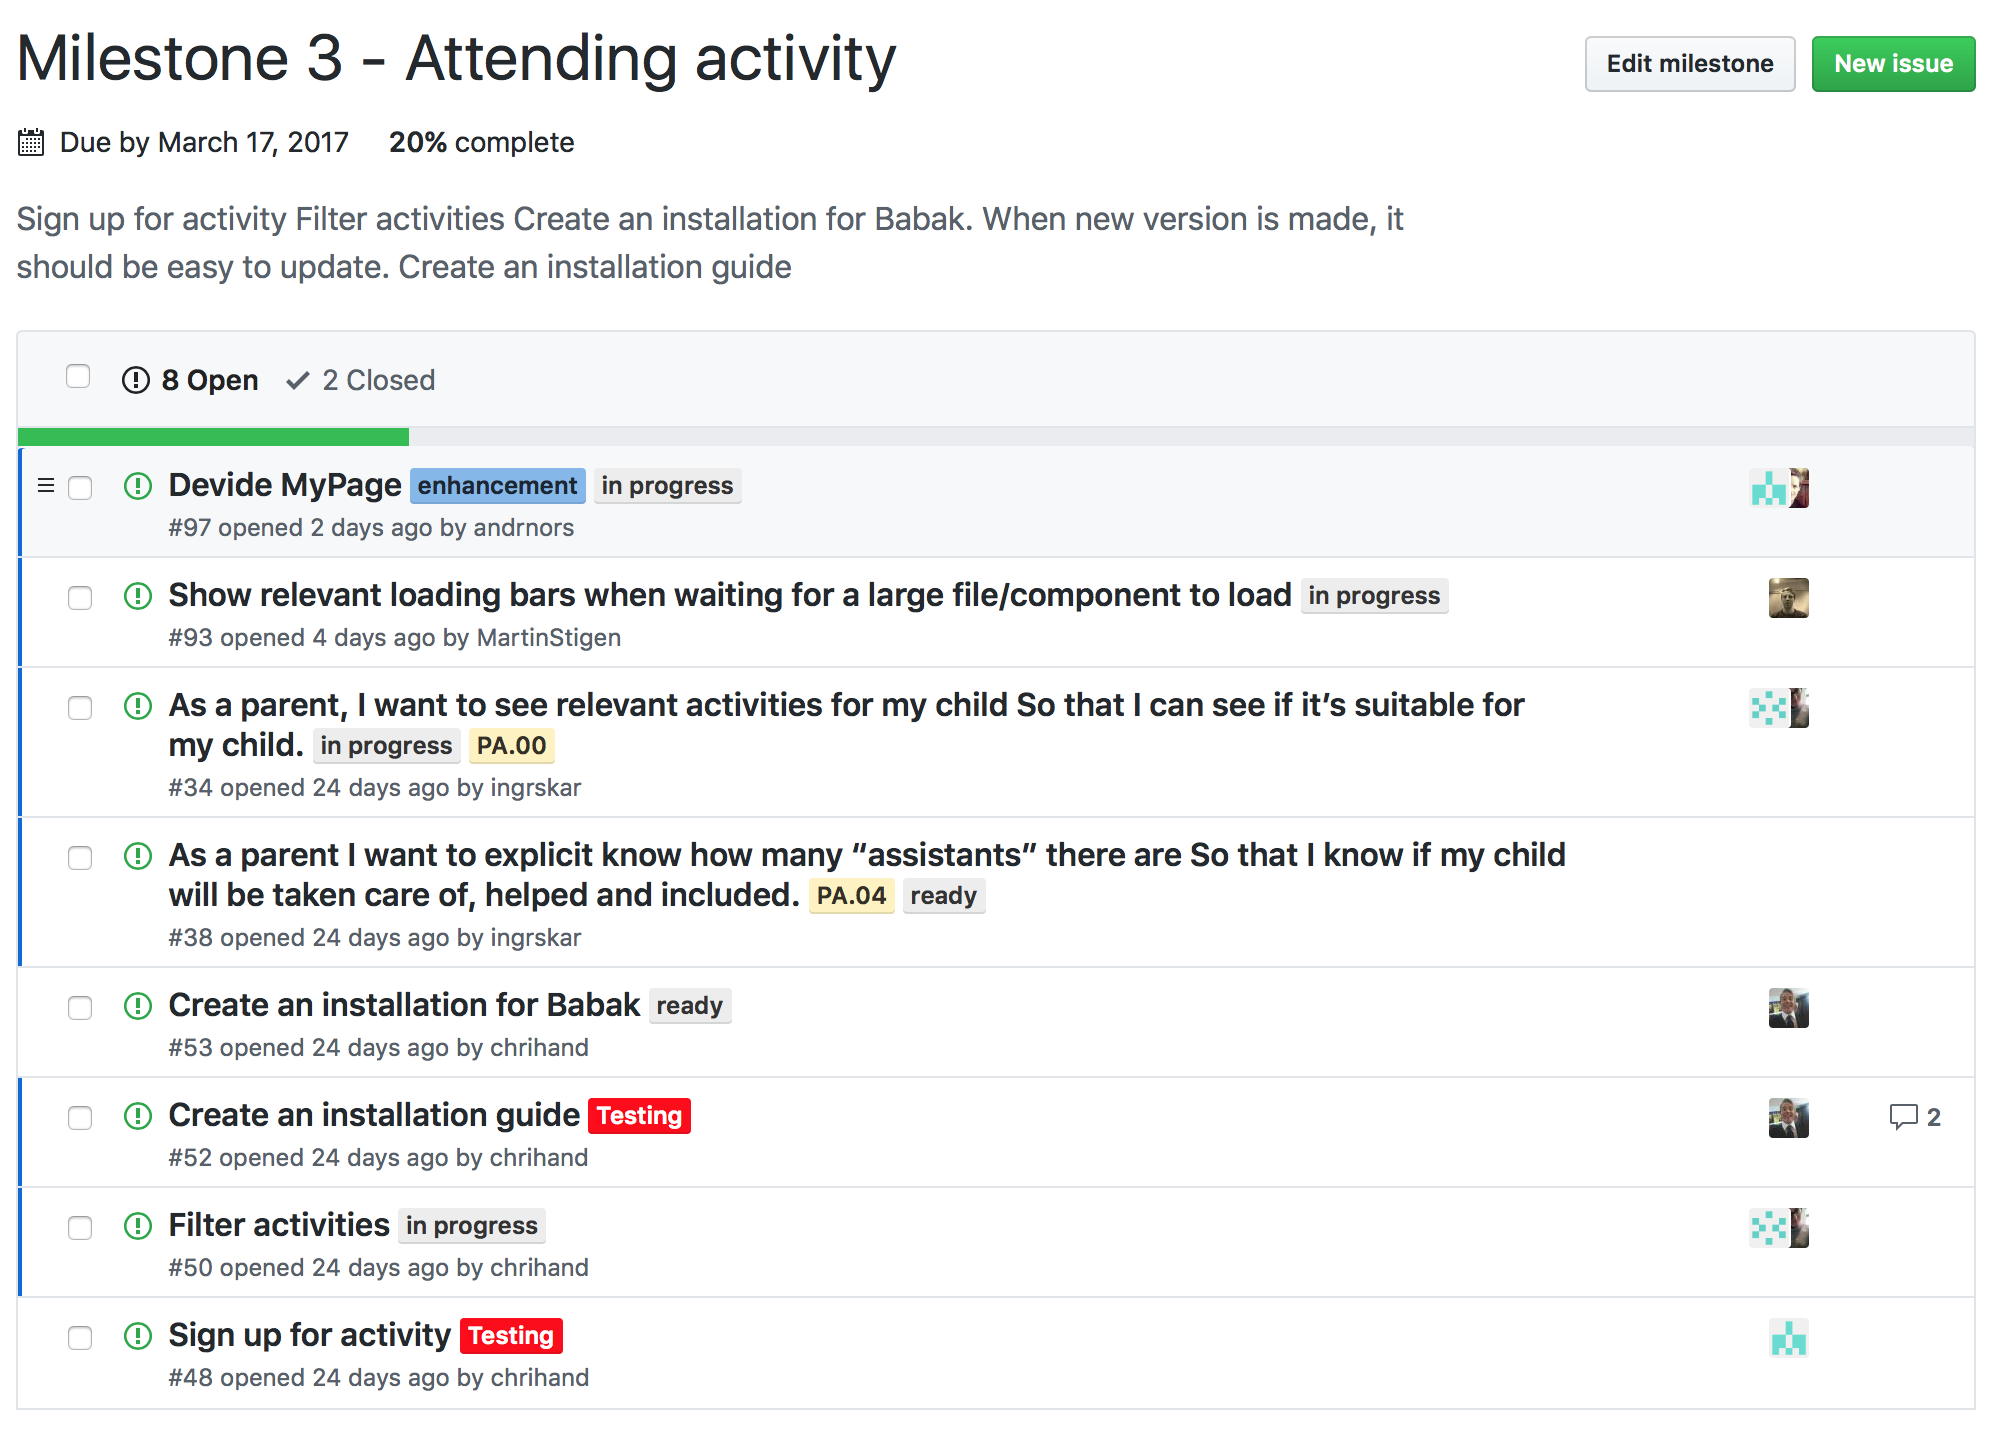
\includegraphics[width=\linewidth, height=80mm]{fig/open_issues}
\caption{Milestone 3 - Open Issues}
\label{Open Issues}
\end{figure}

\begin{figure}[ht]
\centering
    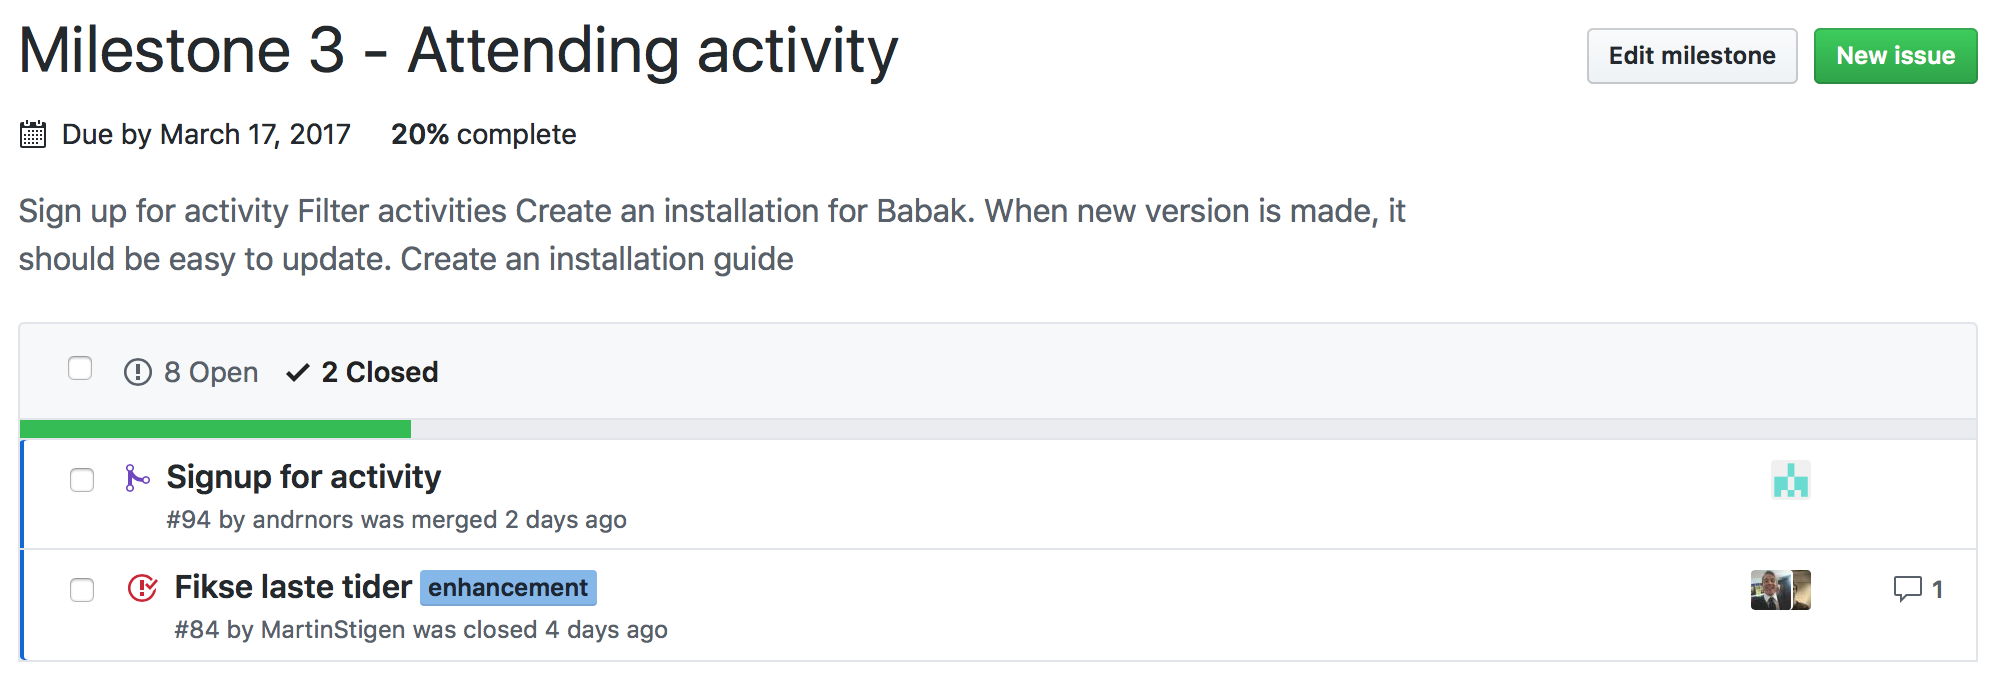
\includegraphics[width=\linewidth, height=45mm]{fig/closed_issues}
\caption{Milestone 3 - Closed Issues}
\label{Closed Issues}
\end{figure}

\section{Risk Analysis} 
\label{riskAnalysis}
The initial risk analysis (see table \ref{risk_analysis}) was created during sprint 0. The cases and their values were mainly based on experience from previous projects. During the development of the project they were adapted by thoroughly going through each case collaboratively, doing new evaluations. Updates made to the risk analysis can be found in section \ref{updated_risk_analysis}. 

Each risk was evaluated and given a number between 1 and 9. One is considered minimal likelihood to occur, and 9 is very likely to occur. The risks were then arranged according to importance and sorted in descending order. The preventive actions are the actions the group carried out to prevent the risks of happening. If a risk occurred, the group considered the remedial action to solve the case at hand. 

\begin{longtable}{@{\extracolsep{\fill}}
                |L{0.14\linewidth}
                |L{0.09\linewidth}
                |L{0.09\linewidth}
                |L{0.14\linewidth}
                |L{0.17\linewidth}
                |L{0.17\linewidth}|@{}}
\hline

\rowcolor{Gray}
\textbf{Description} & \textbf{Likelihood (1-9)} & \textbf{ Impact (1-9)} & \textbf{Importance {\footnotesize (Likelihood * Impact)}} & \textbf{Preventive Action}    & \textbf{Remedial Action} \\ \hline


Conflicts within group & 7 & 7 & 49 & Talk together, give constructive feedback & Try to resolve it with a neutral third party \\
\hline
Unrealistic goals & 7 & 6 & 42 & Talk to customer, be realistic & Be flexible and change goals \\
\hline
Falling Behind Schedule & 6 & 6 & 36 & Daily stand-up meetings, be efficient at meetings, have scheduled meetings & Re-estimate workload, increase work hours \\
\hline
Sickness & 8 & 4 & 32 & Eat healthy, be hygienic & Stay at home, if possible work from home \\
\hline
Technical challenges & 5 & 6 & 30 & Think ahead, test early, build modular & Reconsider technical choices, contact people with knowledge \\
\hline
Lack of knowledge & 9 & 3 & 27 & Be prepared, read up on topic/tech & Ask for help, read about the topics we lack knowledge about \\
\hline
Merge conflicts & 8 & 3 & 24 & Always pull from master before branching & Solve it, run unit tests after resolving conflict \\
\hline
Absent customer & 3 & 7 & 21 & Have scheduled meetings & Refer to customer contract \\
\hline
Lack of communication in group & 5 & 4 & 20 & Slack and meetings & Talk to group representative \\
\hline
Lack of responsibility & 3 & 6 & 18 & Daily stand-up meetings, follow up on given tasks, collaborative work hours & Group leader’s responsibility to follow up \\
\hline
Inefficient meetings & 8 & 2 & 16 & Follow the meeting agenda, strict group leader, bring coffee & Take breaks \\
\hline
Late Arrivals & 8 & 2 & 16 & Give reminders, use the calendar & Bring cake to the group, contact supervisor if it repeats \\
\hline
Data loss & 2 & 6 & 12 & Save often, use git, commit and push often, have local copies & Increase workload, redo work \\
\hline
Poor execution of methodology & 4 & 3 & 12 & Strict group leader, Scrum master, quick recap of methodology & Recap of methodology \\
\hline
Absence & 2 & 5 & 10 & Give reminders, use the calendar & Bring cake to the group, contact supervisor if it repeats \\
\hline
Disagreement of priorities & 5 & 2 & 10 & Everyone gets the opportunity to say what they mean & Talk to customer \\
\hline
Loss of group members & 1 & 9 & 9 & Group representative, social activities & Distribute workload equally over the entire team, adjust goals of project \\
\hline
\caption{Risk Analysis}
\label{risk_analysis}
\end{longtable}

\cleardoublepage